\documentclass{article}


\usepackage[margin=0.6in]{geometry}
\usepackage{amssymb, amsmath, amsfonts}
\usepackage{tabularx}
\usepackage{arydshln}
\usepackage{mathtools}
\usepackage{changepage}
\usepackage{asymptote}
\usepackage{cancel}
\usepackage{physics}
\usepackage{pgf}
\usepackage{enumerate}
\usepackage{placeins}
\usepackage{nth}
\usepackage{array}
\usepackage{tikz}
\usetikzlibrary{arrows,automata}
\tikzset{
  saveuse path/.code 2 args={
    \pgfkeysalso{#1/.style={insert path={#2}}}%
    \global\expandafter\let\csname pgfk@\pgfkeyscurrentpath/.@cmd\expandafter\endcsname
      % not optimal as it is now global through out the document
                           \csname pgfk@\pgfkeyscurrentpath/.@cmd\endcsname
    \pgfkeysalso{#1}},
  /pgf/math set seed/.code=\pgfmathsetseed{#1}}
\usepackage{nicefrac}
\usepackage{pgfplots}
\usepgfplotslibrary{polar}
\pgfplotsset{holdot/.style={fill=white,only marks,mark=*}}
\pgfplotsset{soldot/.style={only marks,mark=*}}
\newcommand{\enth}{$n$th}
\newcommand{\Rl}{\mathbb{R}}
\newcommand{\Cx}{\mathbb{C}}
\newcommand{\sgn}[1]{\text{sgn}\qty[#1]}
\newcommand{\ran}[1]{\text{ran}\qty[#1]}
\newcommand{\E}{\varepsilon}
\newcommand{\qiq}{\qquad \implies \qquad}
\newcommand{\half}{\nicefrac{1}{2}}
\newcommand{\third}{\nicefrac{1}{3}}
\newcommand{\quarter}{\nicefrac{1}{4}}
\newcommand{\f}[3]{#1\ :\ #2 \rightarrow #3}
\newcommand{\Dx}{\Delta x}
\newcommand{\Dy}{\Delta y}
\newcommand{\Dt}{\Delta t}
\newcommand{\hot}{\text{h.o.t.}}
\newcommand{\centdiff}{\frac{u_j^{n+1} - u_j^n}{\Dt}}
\newcommand{\dod}{Domain of Depdendence}

\newcommand{\tridsym}[3]{
    \qty(\begin{array}{ccccc}
                    #1 & #2 & & & \\
                    #3 & #1 & #2 & & \\
                    & \ddots & \ddots & \ddots &  \\
                    & & #3 & #1 & #2 \\
                    & & & #3 & #1
                \end{array})
}


\DeclareMathOperator*{\esssup}{\text{ess~sup}}

\title{MAT 228B Notes}
\author{Sam Fleischer}
\date{February 27, 2017}

\begin{document}
    \maketitle

    \section{Second Order Methods}
        Consider a space-time grid and the point $(x_j,t_{n+1})$.  Assume $a > 0$ and $\nu \leq 1$.

        \begin{figure}[ht!]
            \centering
            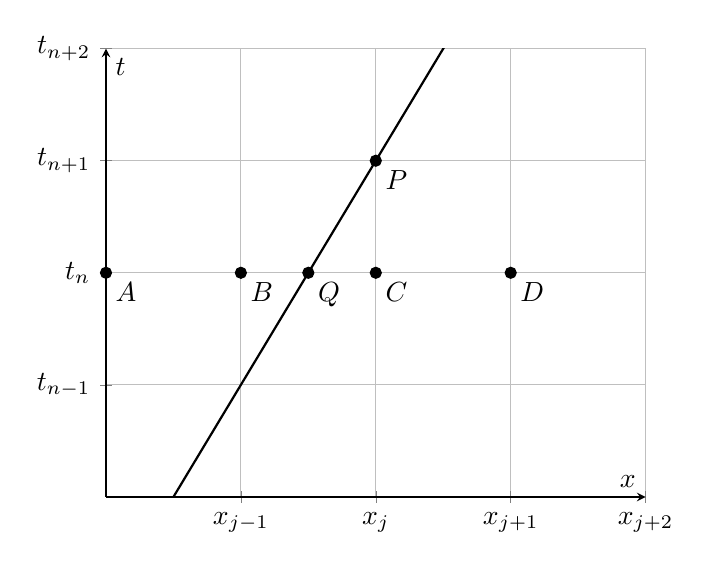
\begin{tikzpicture}
                \begin{axis}[
                  axis lines=middle,
                  grid=major,
                  xmin=2,
                  xmax=6,
                  ymin=2,
                  ymax=6,
                  xlabel=$x$,
                  ylabel=$t$,
                  xtick={3,4,5,6},
                  ytick={3,4,5,6},
                  xticklabels={$x_{j-1}$,$x_j$,$x_{j+1}$,$x_{j+2}$},
                  yticklabels={$t_{n-1}$,$t_n$,$t_{n+1}$,$t_{n+2}$}
                ]
                \addplot[mark=*] coordinates {(4,5)}{};
                \addplot[mark=*] coordinates {(2,4)}{};
                \addplot[mark=*] coordinates {(3,4)}{};
                \addplot[mark=*] coordinates {(4,4)}{};
                \addplot[mark=*] coordinates {(5,4)}{};
                \addplot[mark=*] coordinates {(3.5,4)}{};
                \node at (axis cs:4,5) [anchor=north west] {$P$};
                \node at (axis cs:2,4) [anchor=north west] {$A$};
                \node at (axis cs:3,4) [anchor=north west] {$B$};
                \node at (axis cs:4,4) [anchor=north west] {$C$};
                \node at (axis cs:5,4) [anchor=north west] {$D$};
                \node at (axis cs:3.5,4) [anchor=north west] {$Q$};
                \addplot[domain=0:10,thick] {5 + 2*(x-4)};
                \end{axis}
            \end{tikzpicture}
        \end{figure}

        Use 3 points and quadratic interpolation.  Use points $B$, $C$, and $D$ and get Lax-Wendroff.  or use $A$, $B$, and $C$ to get Mean-Warming which gives $2$nd order upwinding scheme and/or $1$-sided LW.

        Derive LW/BW from Taylor expansion
        \begin{align*}
            u(x, t+\Dt) = u(x+t) + \Dt u_t + \frac{\Dt^2}{2}u_{tt} + \order{\Dt^3}
        \end{align*}
        Then use the PDE to express time derivatives as space derivatives, so
        \begin{align*}
            u_t + au_x = 0 \qquad\qquad\text{means}\qquad\qquad u_t = -au_x
        \end{align*}
        and so $u_{tt} = -au_{tx} = a^2 u_{xx}$, so
        \begin{align*}
            u(x, t + \Dt) = u(x,t) - a\Dt u_x + \frac{a^2\Dt^2}{2}u_{xx} + \order{\Dt^3}
        \end{align*}
        Now use finite differences to approximate the spatial derivatives.  If we use centered second-order differences, we get the Lax-Wendroff method:
        \begin{align*}
            u_j^{n+1} = u_j^n - \frac{a\Dt}{2\Dx}\qty(u_{j+1}^n - u_{j-1}^n) + \frac{a^2\Dt^2}{2\Dx^2}\qty(u_{j+1}^n - 2u_j^n + u_{j-1}^n)
        \end{align*}

        We can use one-sided differences (upwind) for $a > 0$.  So we get the Beam Warming scheme.

        LW is
        \begin{align*}
            \frac{u_j^{n+1} - u_j^n}{\Dt} + \frac{a}{2\Dx}\qty(u_{j+1}^n - u_{j-1}^n) = \frac{a^2\Dt}{2\Dx^2} = \frac{a^2\Dt}{2\Dx^2}\qty(u_{j-1}^n - 2u_j^n + u_{j+1}^n)
        \end{align*}
        Truncation error analysis:
        \begin{align*}
            u_t + \frac{\Dt}{2}u_{tt} + \order{\Dt^2} + au_x + \order{\Dx^2} = \frac{a^2}{\Dt}{2}u_{xx} + \order{\Dt\Dx^2} \\
            u_{tt} = a^2u_{xx}
        \end{align*}
        and the $\text{LTE} = \order{\Dt^2} + \order{\Dx^2}$.

        For Beam Warming,
        \begin{align*}
            u_t = \frac{\Dt}{2}u_{tt} + \order{\Dt^2} + au_x + \order{\Dx^2} = \frac{a^2\Dt}{2}u_{xx} + \order{\Dt\Dx}
        \end{align*}
        and so
        \begin{align*}
            \text{LTE} = \order{\Dt^2} + \order{\Dx^2} + \order{\Dt\Dx}
        \end{align*}
        Stability of Lax-Windroff:
        \begin{align*}
            \abs{g(\xi)}^2 = \abs{-4\nu^2\qty(1 - \nu^2)\sin^4(\frac{\xi\Dx}{2})}
        \end{align*}
        So we require $4\nu^2\qty(1 - \nu^2) \geq 0$ for stability.  So we need $\nu^2 \leq 1$.  And again, we get $\dfrac{\Dt\abs{a}}{\Dx} \leq 1$.

\end{document}












